\documentclass[twocolumn]{article}
\usepackage[utf8]{inputenc}
\usepackage{enumerate}
\usepackage{amsmath}
\usepackage{mathtools}
\usepackage{graphicx}
\usepackage{listings}
\linespread{1.05}
\usepackage[sc]{mathpazo}
\usepackage{color}
\usepackage{gensymb}
\usepackage{multicol}
\usepackage{ltxgrid}
\usepackage{float}
\usepackage{romannum}
\usepackage{times}
\usepackage{subfigure}
\usepackage{subcaption}


\begin{document}
\title{\vspace{-2.5cm}FYS3150 Project 4}
\author{Tobias Berdiin Olesen}
\date{November 2017}
\maketitle
\onecolumngrid
\noindent\makebox[\linewidth]{\rule{\paperwidth}{0.4pt}}
\begin{center}
\section*{Abstract}
Assuming circular orbits for the planets in the solar system gave a decent approximation of the planets trajectories. The verlet algorithm produced more precise values than the euler method which was not able to conserve the energy and angular momentum nor the planets orbits run over a larger time period. The perihelion angle of mercury found is in good agreement with the prediction made by the general theory of relativity. The angle found was $0.11924\degree$ and lies within $99.8\%$ of the observed value. 
\end{center}

\noindent\makebox[\linewidth]{\rule{\paperwidth}{0.4pt}}
\newline
\twocolumngrid

\section{INTRODUCTION}
The aim of this project is to study a model to simulate phase transitions, namely the popular Ising model in two dimensions. This model is widely used, with applications spanning from studies of phase transitions to simulations in statistics.\newline
The purpose of this model (as with all models) is to reduce the complexity of the problem while at the same time retaining the essential physics of the system. The Ising model does this very effectively.
More precisely I will use the Ising model to investigate the properties of a two dimensional ferromagnetic material (like iron) at varying temperatures and for different lattice sizes.
In one and two dimensions the Ising model has analytical solutions to several expectation values, so it gives a qualitatively good understanding of several types of phase transitions.\newline

At a given critical temperature, the Ising model exhibits a phase transition from a magnetic phase (a system with finite magnetic moment) to a phase with zero magnetization. This is a binary system where the objects at each lattice site can only take two values, and here I will use spins pointing up or down as the model for the system.\newline
I will start by assuming we have a simple 2x2-lattice with two spins in each direction, and then find analytical expressions for the partition function and the corresponding expectation values for the energy E, the mean absolute value of the magnetic moment $|M|$ (which I sometimes will refer to as the mean magnetization), the specific heat capacity $C_v$ and the magnetic susceptibility $\chi$ as functions of the temperature T using periodic boundary conditions. These results will serve as benchmark calculations for my numerical calculations later, in order to test if our code and numerical algorithms are giving us correct result to satisfactory precision. The algorithm of choice for solving the Ising model is the Metropolis algorithm, which is a central algorithm in the Monte Carlo methods.\newline
Furthermore I will discuss the numerical results in depth, and plot the various relevant parameters.
Because of the many time consuming calculations needed to do in this project I will also implement parallelization in my program.

\section{BACKGROUND}
\subsection{Ferromagnetic materials}
In most ordinary materials the magnetic dipoles associated with the atoms have a random orientation. This random distribution of magnetic moment results in approximately zero (macroscopic) magnetic moment. However, in ferromagnetic materials (like iron), a net magnetic moment is produced as a result of the prefered alignment of the atomic spins.
Spin is a quantum mechanical property of the electron (this is not the only particle that has spin though), and can only be in two different states: pointing up or down. The spin of the electrons in atoms are the source of ferromagnetism, and when many of these spins point in the same direction, it creates a net macroscopic magnetic field.
The fact that the spins in ferromagnetic materials 'prefer' to be in alignment is based on two fundamental principles: energy minimization and entropy maximization.

\subsection{Phase transitions}
The point where a phase transition takes place is called a critical point and the associated temperature is called the critical temperature $T_C$. The disappearance of a spontaneous magnetization is a typical example of a second-order phase transition. The behaviour around the critical point can be related to the thermodynamical potential Helmholtz' free energy
\begin{equation}
    F = \langle E \rangle - TS = - k_B TlnZ
\end{equation}
where Z is the partition function of the system, T is the temperature, $k_B$ is the Boltzmann constant and S is the entropy. For simplification I will in the whole project use $k_B = 1$. This expression for F shows in a very clear way the 'struggle' between rise in entropy (from the second law of thermodynamics) and the principle of energy minimization.\newline
Then the specific heat $C_V$ is defined via the second derivative of F: $C_V = - \frac{1}{k_B T^2}\frac{\partial^2(\beta F)}{\partial \beta ^2}$, where $\beta = \frac{1}{k_B T}$. The Ising model exhibits a second order phase transition since the heat capacity diverges. The same goes for the magnetic susceptibility $\chi$. $\chi$ can also be expressed as a second order derivative of F, and it too will diverge at the critical point.\newline
$C_V$ is the heat needed to be added to (or removed from) a system to cause a given temperature change, while $\chi$ describes a material's response to an applied magnetic field. Both $C_V$ and $\chi$ will be affected when $T_C$ is reached.

\subsection{Monte Carlo methods}
Numerical methods known as Monte Carlo methods can loosely be described as statistical simulation methods, which utilizes random numbers to perform the simulation. The physical process is simulated directly, and the only requirement is that the system can be described by a probability distribution function (PDF). The Monte Carlo simulation then does random samplings from the PDF. This selection of random states need to be done appropiately according to the PDF at hand though.

\section{FORMALISM/METHOD}
\subsection{The Ising model}
The Ising model illustrates the system in two dimensions by placing spins (pointing either up or down) at regular lattice points, as shown in figure 1. Every different configuration of spins in the lattice is a microstate, and  the total sum of all the the microstates in the system I may call the multiplicity. The lattice is squared with dimensions $L \times L = N$, where L is the number of spins in each direction and the total number of spins are equal to N. Since each spin has two different directions to be in, the number of possible different configurations of the system is equal to $2^N$. The interactions between the spins are restricted to nearest neighbors only.\newline
With no external magnetic field present the energy for a specific configuration (state) i is given as:
\begin{equation}
    E_i = -J \sum_{<kl>}^{N} s_k s_l
\end{equation}
where the symbol $<kl>$ indicates that the sum is over nearest neighbors only, $s_k$ and $s_l$ are the respective nearest neighbour spins. In my discussion the values for the spins will be +1 for spin up and -1 for spin down. J is a coupling constant expressing the strength of the interaction between neighboring spins. For ferromagnetic materials, $J > 0$, and in this project I will work with $J = 1$. It is from (1) easy to see that it is energetically favorable for neighboring spins to be aligned. This fact can lead to the lattice having a net magnetization even in the absence of a magnetic field.\newline
The magnetization $M_i$ associated with state $i$ is given by:
\begin{equation}
    M_i = \sum_{i}^{N}s_i
\end{equation}

In the case of small systems, the way we treat the spins at the ends of the lattice matters. In this project I will use periodic boundary conditions. This means that the spins at the edges of the lattice are made to interact with the spins at the geometric opposite edges of the lattice.\newline

\begin{figure}[h!]
  \centering
  \caption{One possible configuration of spins in the 2x2 Ising model}
  \includegraphics[width=1.5cm]{2x2-config.png}
\end{figure}

\subsection{Expectation values}
In order to calculate values such as the mean energy $\langle E \rangle$ at a given temperature, I need a probability distribution. This is given by the Boltzmann distribution (more precise this is the probability of finding the system in state $i$):
\begin{equation}
    P_i (\beta) = \frac{e^{-\beta E_i}}{Z}
\end{equation}

with $\beta = \frac{1}{k_B T}$, where T is the temperature, $k_B$ is the Boltzmann constant, $E_i$ is the energy of a microstate $i$ while Z is the partition function defined as:
\begin{equation}
    Z = \sum_{i=1}^{s}e^{-\beta E_i}
\end{equation}
where the sum go over all microstates s. Z is really just a normalization factor which stems from the fact that we need all our probabilities to add up to 1 (the system has to have 'some' finite energy after all):
$$\sum_{i=1}^{s}P_i(\beta) = 1$$
The factors $e^{-\beta E_i}$ is called the Boltzmann factors, so Z is also the sum over the Boltzmann factors.\newline
Now the expectation value for the energy is given by:
\begin{equation}
    \langle E \rangle = \sum_{i=1}^{s}E_i P_i(\beta) = \frac{1}{Z}\sum_{i=1}^{s}E_i e^{-\beta E_i}
\end{equation}
The expectation value for $E^2$ is given by:
\begin{equation}
    \langle E^2 \rangle = \frac{1}{Z}\sum_{i=1}^{s}{E_i}^2 e^{-\beta E_i}
\end{equation}
and the expectation values for the absolute value of the magnetization $|M|$ and $|M|^2$ is defined in the same way. I will use the absolute value of the magnetization instead of the regular magnetization for reasons given in section ??.\newline
The energy $E_i$ and magnetization $M_i$ associated with state $i$ of the system are given by equations (1) and (2).\newline

\subsection{Analytic expressions for the 2x2 case of the Ising model}
As I mentioned in the introduction, the Ising model has analytical solutions to several expectation values in one and two dimensions. Now I will use this fact to find analytical expressions for $\langle E \rangle$, $\langle |M| \rangle$, $C_V$ and $\chi$ for the 2x2 case of the Ising model. To achieve this I will first note that my system has 2 spins in each direction (x and y), which means that the total number of different configurations (or multiplicity) is: $\Omega = 2^N = 2^4 = 16$. This means that I will get 16 (not all distinct) $E_i$- and $M_i$-values. These values are listed in table 1 in the results section.\newline
Then I can find an expression for the partition function Z for the 2x2 case from equation (4) (remember that J=1):
\begin{equation}
    Z = \sum_{i=1}^{\Omega}e^{-\beta E_i} = 12 + 2e^{8\beta} + 2e^{-8\beta}
\end{equation}

$\langle E \rangle$ and $\langle E^2 \rangle$ is found from equation (5) and (6) respectively:

\begin{equation}
\begin{multlined}
    \langle E \rangle = \frac{1}{Z}\sum_{i=1}^{\Omega}E_i e^{-\beta E_i}\\ = \frac{1}{Z}(16e^{-8\beta} - 16e^{8\beta}) = -\frac{32}{Z}\sinh(8\beta)
\end{multlined}
\end{equation}

\begin{equation}
\begin{multlined}
    \langle E^2 \rangle = \frac{1}{Z}\sum_{i=1}^{\Omega}{E_i}^2 e^{-\beta E_i}\\ = \frac{1}{Z}( 128e^{8\beta} + 128e^{-8\beta} ) = \frac{256}{Z}\cosh(8\beta)
\end{multlined}
\end{equation}

where I have used that $cosh(x)=\frac{e^x + e^{-x}}{2}$ and $sinh(x)=\frac{e^x - e^{-x}}{2}$.

The expectation values of the magnetization is as mentioned defined in a similar way as for the energy:

\begin{equation}
    \langle |M| \rangle = \frac{1}{Z}\sum_{i=1}^{\Omega}M_i e^{-\beta E_i} = \frac{1}{Z}( 16 + 8e^{8\beta} )
\end{equation}

\begin{equation}
    \langle |M|^2 \rangle = \frac{1}{Z}\sum_{i=1}^{\Omega}{M_i}^2 e^{-\beta E_i} = \frac{1}{Z}( 32 + 32e^{8\beta} )
\end{equation}

The magnetic susceptibility $\chi$ and specific heat capacity $C_V$ are then found via $\langle E \rangle$ and $\langle |M| \rangle$:

\begin{equation}
    \chi = \frac{1}{k_B T}( \langle |M|^2 \rangle - {\langle |M| \rangle}^2 )
\end{equation}

\begin{equation}
    C_V = \frac{1}{k_B t^2}( \langle E^2 \rangle - {\langle E \rangle}^2 )
\end{equation}

It is also worth noting that:\newline
$\langle M \rangle = \frac{1}{Z}\sum_{i=1}^{\Omega}M_i e^{-\beta E_i} = 0$,
which doesn't really give me any information that I am interested in. That is why I use the absolute value of M in my calculations of the expectation values.

\subsection{The Metropolis algorithm}
The algorithm I will use for solving the Ising model numerically is the Metropolis algorithm. New configurations are generated from a previous one using a transition probability that depends on the energy difference between the initial and final states.\newline

In our case the Monte Carlo sampling function will be the probability of finding the system in a state given by equation (2). The partition function Z is difficult and cumbersome to calculate because we need all the states with all the associated energies to do it. The number of different configurations of spins, and thereby states, is given by $2^N$ since all N spins (as mentioned) can point either up or down. Fortunately, the Metropolis algorithm considers only the ratios between probabilities and we do not need to compute the partition function at all because it cancels out.\newline

The Metropolis algorithm goes as follows:\newline
1. Establish an initial state  with initial energy and magnetization $E_0$ and $M_0$.\newline
2. Change the initial spin configuration, and thereby make a new state, by flipping one of the spins. Which one gets flipped is chosen by random using a random number generator.\newline
3. Calculate the energy difference $\Delta E = E_{new} - E_0$ between the new state and the old. Fortulately, the number of $\Delta E$-values is limited to five for the Ising model in two dimensions. This means that I can precalculate these values in order to reduce the number of FLOPS in my code and thereby the time it takes to run.\newline
4. If $\Delta E \leq 0$ the new configuration will be accepted. The energy is now lowered and we are hopefully moving towards the energy minimum at a given temperature. Go to step 7.\newline
5. If $\Delta E > 0$, calculate $w = e^{-\beta \Delta E}$.\newline
6. Compare w with a random number r. If $r \leq w$, accept the new configuration, else we keep the old configuration.\newline
7. Now update the necessary expectation values (E and M).\newline
8. The steps 2 - 7 are then repeated in order to obtain a sufficiently good representation of states.\newline

Each sweep through the lattice (sum over all spins) constitutes a Monte Carlo cycle. One cycle can be thought of as a measurement. In the end I will divide the various expectation values with number of cycles to 'eliminate' the number of cycles as a factor in the calculations. I will also divide all results by the number of spins.\newline
The energy difference between two states is given by:
\begin{equation}
\begin{multlined}
\Delta E = E_{new} - E_0 = J \sum_{<kl>}^{N} s_{k,1}s_{l,1} - J\sum_{<kl>}^{N} s_{k,2}s_{l,2}\\ = -J \sum_{<kl>}^{N} s_{k,2}(s_{l,2} - s_{l,1})
\end{multlined}
\end{equation}

My numerical results for the relevant parameters in the 2x2 case are listed in tables 3-5, and the analytical results are listed in table 2.
\newline

The number of accepted configurations is plotted by counting every time the requirement in step (4) - (6) is satisfied.\newline

To see the distribution between the different microstates in my system I also plot the probability of a given state occuring, as a function of the associated discrete energy of the state. This is shown in figures 11-14. I find the probabilities by simply counting the times a spesific energy occurs in my simulation, and then dividing by the total number of possible energies.\newline

I also want to study the behaviour of the Ising model close to the  critical temperature. This is done by plotting all the relevant parameters $\langle E \rangle$, $\langle |M| \rangle$, $\chi$ and $C_V$ as functions of temperature, for T $\epsilon[2.1, 2.4]$ with a temperature step of 0.05, and for different lattice sizes L. These plots are shown in figures ??.\newline

From this these results it is possible to read the critical temperatures $T_C(L)$ directly of the plots because the divergence of $C_V$ and $\chi$ at the critical point will be visible in the plots as a discontinuity in the functions.\newline
This makes me able to determine the critical temperature in the thermodynamic limit $L \rightarrow \infty$ from the equation below:
\begin{equation}
    T_C(L) - T_C(L=\infty) = aL^{-1/\nu}
\end{equation}
which gives:
\begin{equation}
    T_C(L=\infty) = T_C(L) - \frac{a}{L}
\end{equation}
where I have used that $\nu = 1$.\newline

The "eye-balling" method for determining $T_C$ is probably not the most accurate though. A better way may be to extract the critical temperatures for each of the lattice sizes numerically, and then plot them with a linear regression as done in figure 12. Because my units on the x-axis here is 1/L, the approximation of the critical temperature in the thermodynamic limit is simply equal to the point where the linear function intersects with the y-axis.

\section{IMPLEMENTATION}
My code is available at my Github adress:\newline

The code was parallized using MPI. Because I have four processors on my computer, this means that I will be able to produce four times the amount of data (that I would have without the parallelization) in the same amount of time. The increase in data points make my results more accurate.
\newpage
\onecolumngrid
\begin{center}
\section{RESULTS}
\end{center}
I refer to temperature as T and number of Monte Carlo cycles as mcs.\newline

\centering\subsection{2x2 case}

\begin{center}
\textbf{Oppg a: Table 1: Possible E- and M-values for the 2x2 case with T=1}
\newline
\bigskip
\resizebox{3cm} {
\centering\begin{tabular}{|| l | l | l | l ||}
    \hline
    Number of spins up & Degeneracy & E & M\\
    \hline 
    4 & 1 & -8J & 4 \\
    \hline
    3 & 4 & 0 & 2 \\
    \hline
    2 & 4 & 0 & 0 \\
    \hline
    2 & 2 & 8J & 0 \\
    \hline
    1 & 4 & 0 & -2\\
    \hline
    0 & 1 & -8J & -4 \\
    \hline
\end{tabular}
}\newline
\end{center}

%Analytiske forventningsverdier tabell:
\textbf{Oppg a: Table 2(below): Analytical expectation values for the 2x2 case with T=1}
\newline
\centering
\bigskip
\resizebox{3cm} {
\begin{tabular}{|| l | l | l | l | l | l ||}
    \hline
    $\langle E \rangle$ & $\langle E^2 \rangle$ & $\langle |M| \rangle$ & $\langle |M|^2 \rangle$ & $\chi$ & $C_V$\\
    \hline 
    -1.995980 & 15.96790 & 0.998661 & 3.993300 & 0.016043 & 0.128329 \\
    \hline
\end{tabular}
}


\newpage

\begin{table}
\centering
\caption{Numerical expectation values for the 2x2 case with T=1 and mcs=100}
\begin{tabular}{l | l | l | l | l | l | l}
    \hline
    \hline
    $\langle E \rangle$ & $\langle E^2 \rangle$ & $\langle |M| \rangle$ & $\langle |M|^2 \rangle$ & $\chi$ & $C_V$ & $\sigma^2$(variance)\\
    \hline 
    -1.98 & 15.84 & 0.9925 & 3.965 & 0.0991 & 0.6336 & 0.1584 \\
    \hline
    \hline
\end{tabular}
\end{table}
\centering
\textbf{Oppg b: Table 4: Numerical expectation values for the 2x2 case with T=1 and mcs = 10000000}
\newline
\bigskip
\resizebox{3cm} {
\begin{tabular}{|| l | l | l | l | l | l | l ||}
    \centering
    \hline
    $\langle E \rangle$ & $\langle E^2 \rangle$ & $\langle |M| \rangle$ & $\langle |M|^2 \rangle$ & $\chi$ & $C_V$ & $\sigma^2$(variance)\\
    \hline 
    -1.99596 & 15.9677 & 0.99865 & 3.99326 & 0.0162153 & 0.129 & 0.0322499 \\
    \hline
\end{tabular}
}
\centering
\textbf{Oppg b: Table 5: Numerical expectation values for the 2x2 case with T=1 and mcs = 1000000000}
\newline
\centering
\bigskip

\resizebox{3cm} {
\begin{tabular}{|| l | l | l | l | l | l | l ||}
    \hline
    $\langle E \rangle$ & $\langle E^2 \rangle$ & $\langle |M| \rangle$ & $\langle |M|^2 \rangle$ & $\chi$ & $C_V$ & $\sigma^2$(variance)\\
    \hline 
    -1.99598 & 15.9679 & 0.998661 & 3.9933 & 0.0160384 & 0.128333 & 0.0320833 \\
    \hline
\end{tabular}
}

\centering\subsection{Plots of number of accepted configurations}

\begin{figure}[h!]
  \centering
  \caption{Oppg c:Plot of accepted configurations vs mcs, for T = 1.0 and mcs = 1000, 20x20 spins and an ordered starting configuration}
  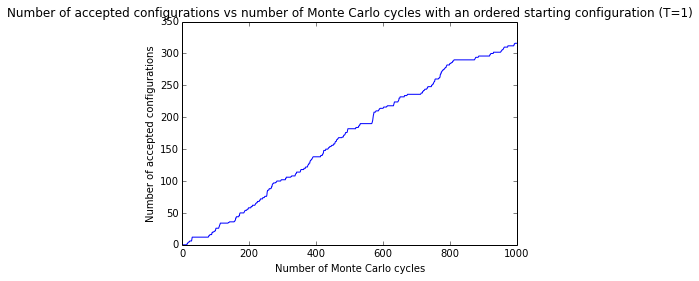
\includegraphics[width=10cm]{configs_plot_1.png}
\end{figure}

\begin{figure}[h!]
  \centering
  \caption{Oppg c: Plot of accepted configurations vs mcs, for T = 2.4 and mcs = 1000. 20x20 spins and an ordered starting configuration}
  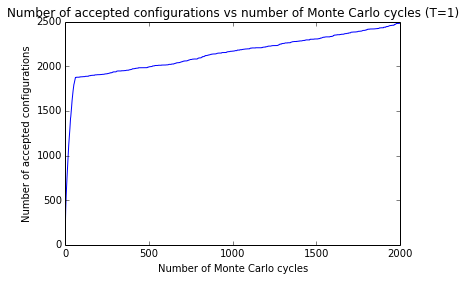
\includegraphics[width=10cm]{configs_plot_2.png}
\end{figure}

\begin{figure}[h!]
  \centering
  \caption{Oppg c: Plot of accepted configurations vs mcs, for T = 1.0 and mcs = 1000, 20x20 spins and a random starting configuration.}
  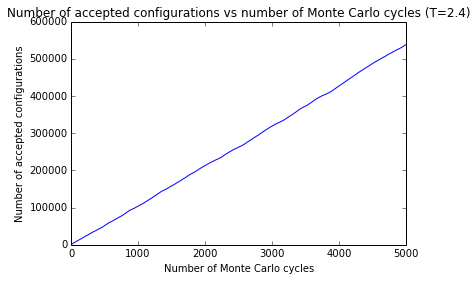
\includegraphics[width=10cm]{configs_plot_3.png}
\end{figure}
\newpage

\newpage

\centering\subsection{Energy and magnetization plots}

\newpage

\newpage

\begin{figure}[h!]
  \centering
  \caption{Oppg c: Plot of energy and magnetization as function of mcs, for T=1 and 20x20 spins with a random starting configuration}
  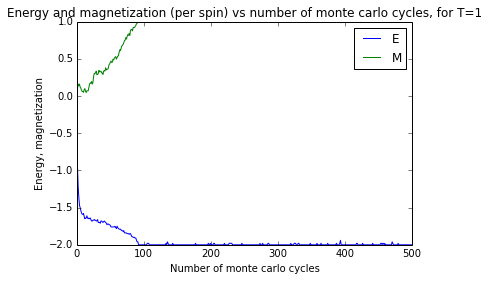
\includegraphics[width=10cm]{E_M_plot_c_1.png}
\end{figure}

\begin{figure}[h!]
  \centering
  \caption{Oppg c: Plot of energy and magnetization as function of mcs, for T=2.4 and 20x20 spins with a random starting configuration}
  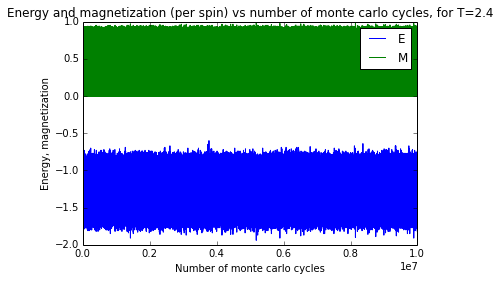
\includegraphics[width=10cm]{E_M_plot_c_2.png}
\end{figure}

\begin{figure}[h!]
  \centering
  \caption{Oppg c: Plot of energy and magnetization as function of mcs, for T=1 and 20x20 spins with an ordered starting configuration}
  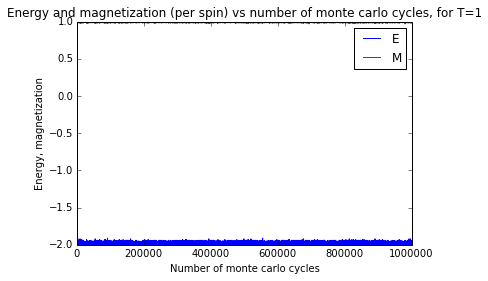
\includegraphics[width=10cm]{E_M_plot_c_3.png}
\end{figure}

\begin{figure}[h!]
  \centering
  \caption{Oppg c: Plot of energy and magnetization as function of mcs, for T=2.4 and 20x20 spins with an ordered starting configuration}
  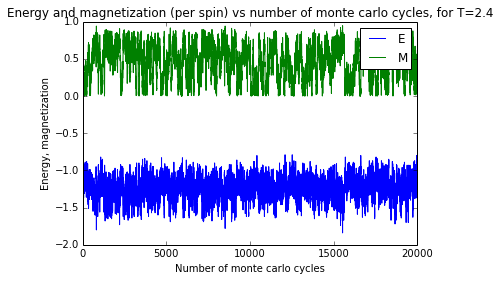
\includegraphics[width=10cm]{E_M_plot_c_4.png}
\end{figure}

\centering\subsection{Plots of probability functions}

\begin{figure}[H]
  \centering
  \caption{Oppg d: Plot of the probabilities for discrete energy values near equilibrium, for T=1, mcs = 1000000, E-variance=11.54 and 20x20 spins with a random starting configuration}
  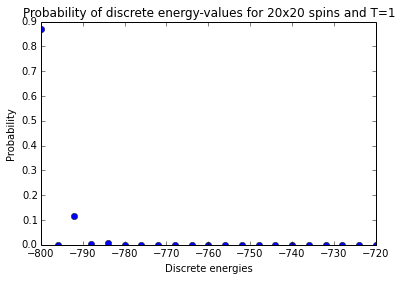
\includegraphics[width=10cm]{FYS3150_Proj4d_plot.png}
\end{figure}

\begin{figure}[h!]
  \centering
  \caption{Oppg d: Plot of the probabilities for discrete energy values, for T=2.4, mcs = 1000000, E-variance=3242.64 and 20x20 spins with a random starting configuration}
  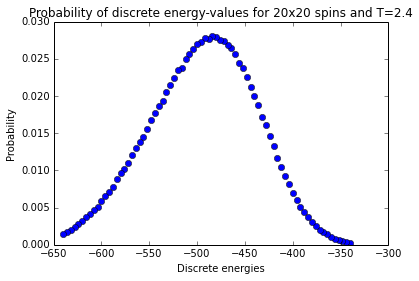
\includegraphics[width=10cm]{FYS3150_Proj4d_2_plot.png}
\end{figure}

\begin{figure}[h!]
  \centering
  \caption{Oppg d: Plot of the probabilities for discrete energy values, for T=2.0, mcs = 1000000, E-variance=1159.75 and 20x20 spins with a random starting configuration}
  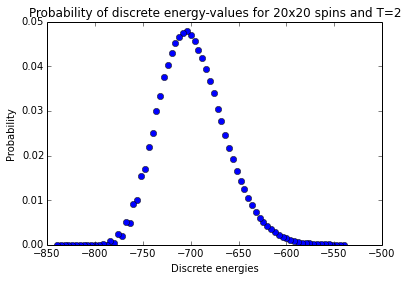
\includegraphics[width=10cm]{FYS3150_Proj4d_3_plot.png}
\end{figure}

\begin{figure}[h!]
  \centering
  \caption{Oppg f: Linear regression over $T_C$-values, for T$\epsilon$[2.1, 2.4], mcs = 1000000 and a random starting configuration.}
  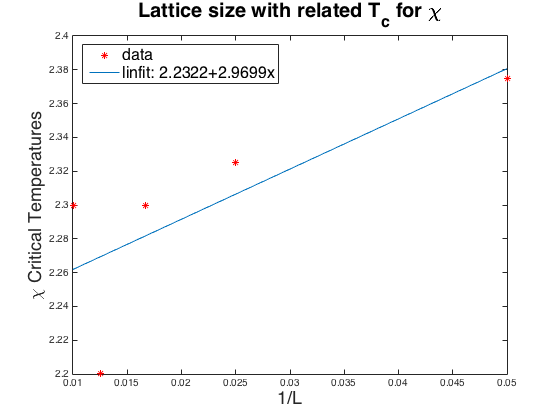
\includegraphics[width=10cm]{Proj4_f_linear_plot.png}
\end{figure}

\newpage
\newpage
\newpage
\newpage
\newpage
\twocolumngrid
\section{DISCUSSION}
\subsection{The 2x2 case}
b):\newline
I will start my discussion by talking about the 2x2 case of the Ising model with temperature T=1. It is clear from looking at tables 2-5 that my numerical results for the expectation values of E, $E^2$ $|M|$ and $|M|^2$ are getting closer and closer to their respective analytical values as the number of Monte Carlo cycles increases. The same goes for the susceptibility and the magnetization. This statement is further supported by the fact that the variance in energy decreases as the number of Monte Carlo cycles increase. For 1000000000 (a billion) Monte Carlo cycles I see a very good agreement between the analytical and the numerical results, with a small variance. A smaller variance means less uncertainty, and thereby more accurate results.\newline

\subsection{The 20x20 case: The behaviour of energy and magnetization}

Moving on to the 20x20 case, I plotted the mean energy and absolute value of the magnetization as a function of Monte Carlo cycles in order to study how many cycles were needed before reaching equilibrium. From figure 5 it is pretty clear that the energy converges to the value of about -2 and the magnetization converges to a value of about 1.\newline

At low temperatures (T=1) and an ordered starting configuration (all spins pointing the same way) I reach a stable value for the energy rather quickly.  
For T=1 and a random starting configuration of spins, both the energy and magnetization still converges pretty quickly towards their respective expectation values, but it takes a little bit longer than for the ordered case. Then they just fluctuate around these values. Equilibrium is reached when the energy has reached it's expectation value (circa). This happens at about the 100th Monte Carlo cycle, as seen from figure 7. This behaviour is as expected.\newline
It is clear from the plots that both the energy and magnetization fluctuates much more and uses longer time to reach the steady state with a higher temperature T=2,4. This makes sense though, because with higher energy comes higher multiplicity: When the temperature increases, the Boltzmann factor allows me to access more states, which increases the probability of accessing other states.\newline
It's easy to see from figures 5 and 6 that with lower temperature, it's much "easier" for the system to reach equilibrium. \newline

In figures 2-4 I have plotted the number off accepted configurations versus the number of monte carlo cycles. By studying figure 4 I see that for a random starting configuration and T = 1, the number of accepted configurations increase greatly in the beginning, but then flattens out at around the 250th mc-cycle. The point where the graph flattens out is the point where the system reaches thermal equilibrium. At this point the system has reached the low energy that it 'wants', as per the principle of energy minimization and equations (1) and (4). This statement is in agreement with the probabilities plotted in figure 9: Here it is evident that the most likely state is by far the ground state, which has the least energy and where the spins are ordered. So the system in figure 4 goes from a random configuration to a more ordered configuration. When the system has reached the steady state, the rate at which new configurations are accepted will slow down and then stay constant. This is because the ground state is overwhelmingly likely compared to any other states at this point.\newline

How an increase in temperature affects the probability distribution of states is evident from figures 9-11, which all illustrates the system with a random initial configuration. The increase in temperature causes an increase in the width of the distribution function, which means that the probabilities are more 'spread out' between the different states.\newline

Comparing figure 2 and 3 is also an interesting exercise. Both these systems have an ordered spin configuration initially, so the only difference between the two plots are the temperature. It is easy to see that for the higher temperature T=2.4, the number of accepted configurations increases much faster than for T=1. This is what one would expect from equations (1) and (4):
Most states now have a more equal probability (as mentioned in my discussion of figures 9-11), and the entropy-term in equation (1) increases.\newline
In general, it takes shorter time for a system to go from an ordered to unordered state, than the other way around.\newline

\subsection{The probability distribution}

The variance $\sigma_E^2$ for the L=20, T=2.4, mcs = 1000000 system with a random starting configuration is: 3242.64. This gives a standard deviation $\sigma_E = \sqrt{\sigma_E^2} = 56.94$. I want to compare this standard deviation value with the full width at half the maximum (FWHM) of the probability plot  in figure 12. I see then that these two values are not in agreement. Reading straight from the plot in figure 12, the width at half the maximum looks to be about 200.\newline
The big difference between these two values are not unexpected though, because at the temperature T=2.4, we are close to the critical temperature $T_C = 2.269$ where the phase transition happens. Because of this, my distribution is not Gaussian anymore, which explains the disagreement.\newline

With the above paragraph in mind, it would then be interesting to lower the temperature in order to get further away from the critical temperature before doing the same comparison again, still with a random starting configuration.\newline
With a temperature T = 2.0, the variance for this case is: $\sigma_E^2$ = 1159.75, which gives a standard deviation of: $\sigma = 34.06$. If I measure by eye the FWHM of the plot in figure 13, I find a width of about 50. This shows a much better agreement, and is as expected.\newline

What has been talked about in the earlier paragraphs and what one can see from both the probability distribution plots and the plots of the expectation values for E and M, is physics governed by the Boltzmann distribution function given in equation (3).\newline

From the plot in figure 14 I see that (the approximation of) $T_C(L=\infty) = 2.2322$, which isn't that far away from the exact result from Lars Onsager: 2.269.\newline

It is also worth mentioning that there exists a correlation between the different spin configurations (microstates) because I only flip one single spin at a time (each time I change the configuration). This correlation shouldn't be too big though, because I still end up flipping $L^2$ spins per Monte Carlo cycle.\newline

\section{CONCLUSION}
From the results I have gotten in this project I can conclude that the Ising model seems to be a good way of explaining the magnetic phenomena in ferromagnetic materials. It seems to replicate experimental results well. 

\section{REFERENCES}
Hjort -Jensen, Morten., 2015. Computational Physics Kompendiet.

\end{document}